% !TEX TS-program = pdflatex
% !TEX encoding = UTF-8 Unicode
% !TEX root = ../main.tex
% !TEX spellcheck = en-US
% ****************************************************************************************
% File: purpose_and_scope.tex
% Author: Patrick Haselwanter
% Date: 2023-10-28
% ****************************************************************************************
\chapter{Package overview}
\label{chapter:package_overview}
The \texttt{turtlesimAutomata} package consists of the following nodes:

\begin{itemize}
    \item \texttt{/start\_turtle} listens to the \emph{/rosout} topic for a message containing "Spawning turtle" which indicates that the \texttt{turtlesim\_node} node has started successfully. It will then send a randomly computed angle to the \texttt{/turn\_turtle} node via the \emph{/turn\_angle} topic and shut itself down afterwards.
    \item \texttt{/drive\_turtle\_continuously} continuously sends a message to the \emph{/turtle1/cmd\_vel} topic to drive the turtle in a straight line. The sending of said message may be toggled via the \emph{/drive\_turtle} topic.
    \item \texttt{/turn\_turtle} listens to the \emph{/turn\_angle} topic for a message containing the angle by which the turtle shall turn. The node includes a client for the \emph{/turtle1/teleport\_relative} service (not visible in \autoref{fig:turtlesimAutomata_nodes}), which is hosted by the \texttt{/turtlesim\_node} and is being used to request a turn of the turtle by the received angle. The node functions mostly as a relay station.
    \item \texttt{/edge} listens to the \emph{/rosout} topic for a message containing "Oh no! I hit the wall!" which is published by the \texttt{turtlesim\_node} node when the turtle reaches the edge of the window. It will then tell the \texttt{/drive\_turtle\_continuously} node to stop driving the turtle forwards, send a message via the \emph{/turn\_angle} topic to request a 90 degree clockwise turn by the \texttt{/turn\_turtle} node and afterwards tells the \texttt{/drive\_turtle\_continuously} node to continue driving the turtle forwards.
\end{itemize}


\begin{figure}[htbp]
    \centering
    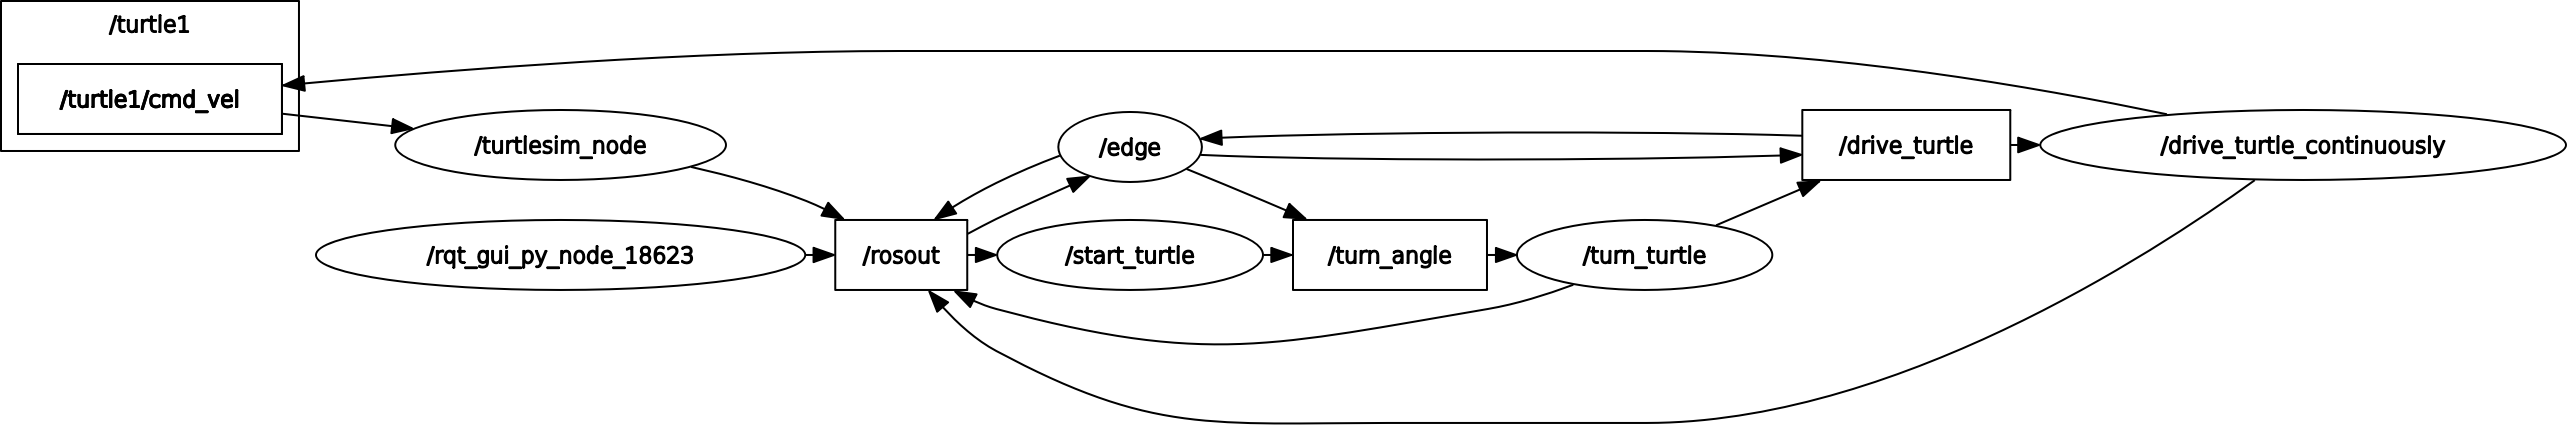
\includegraphics[width=1\textwidth]{./img/rosgraph.png}
    \caption{Nodes and topics of the \texttt{turtlesimAutomata} package shown in \texttt{rqt\_graph}}
    \label{fig:turtlesimAutomata_nodes}
\end{figure}



% EOF